\chapter{FiCSW}
{
  \label{chap:ficsw}
  本章では,FiCシステムとマルチFPGAシステムであるFiCSWの概要を説明する.
  
  \section{FiCの概要}
  \label{sec:about_fic}
  FiCはNEDOのプロジェクトとして以下のようなシステムの構成を目指している.
  
  \begin{enumerate}
    \item 様々な種類の処理装置を適材適所で組み合わせて運用する「異種エンジンシステム」とすることで,汎用プロセッサを遥かに超える演算能力を有する
    \item 光通信技術の導入により,高速通信が可能なインターコネクトを実現することでホストプロセッサを介することなくエンジン同士を接続し通信のオーバーヘッドの小さなシステムを構築すること
  \end{enumerate}
  
  人工知能計算基盤としてのクラウドシステムなので,大量データによる学習フェーズなど即時性を必要としない演算処理を担うことが想定される,
  それに加え,様々なアプリケーションで柔軟にエンジンを効率よく割り当てるためにエンジン間を動的に変更することが
  可能なネットワークを構成する必要がある.
  
  \subsection{FiCのアーキテクチャ}
  \label{sec:arch_fic}
  FiCは3つの基板(ノード)とそれらをつなぐネットワークから構成される.ノードには本研究で用いるFPGAノードだけでなく
  GPUノード,メモリノードがある.これらは図\ref{fig:arch_fic}に示すような接続により計算クラスタとして各種アプリケーションに用いられる.
  
  \begin{figure}[h]
    \centering
    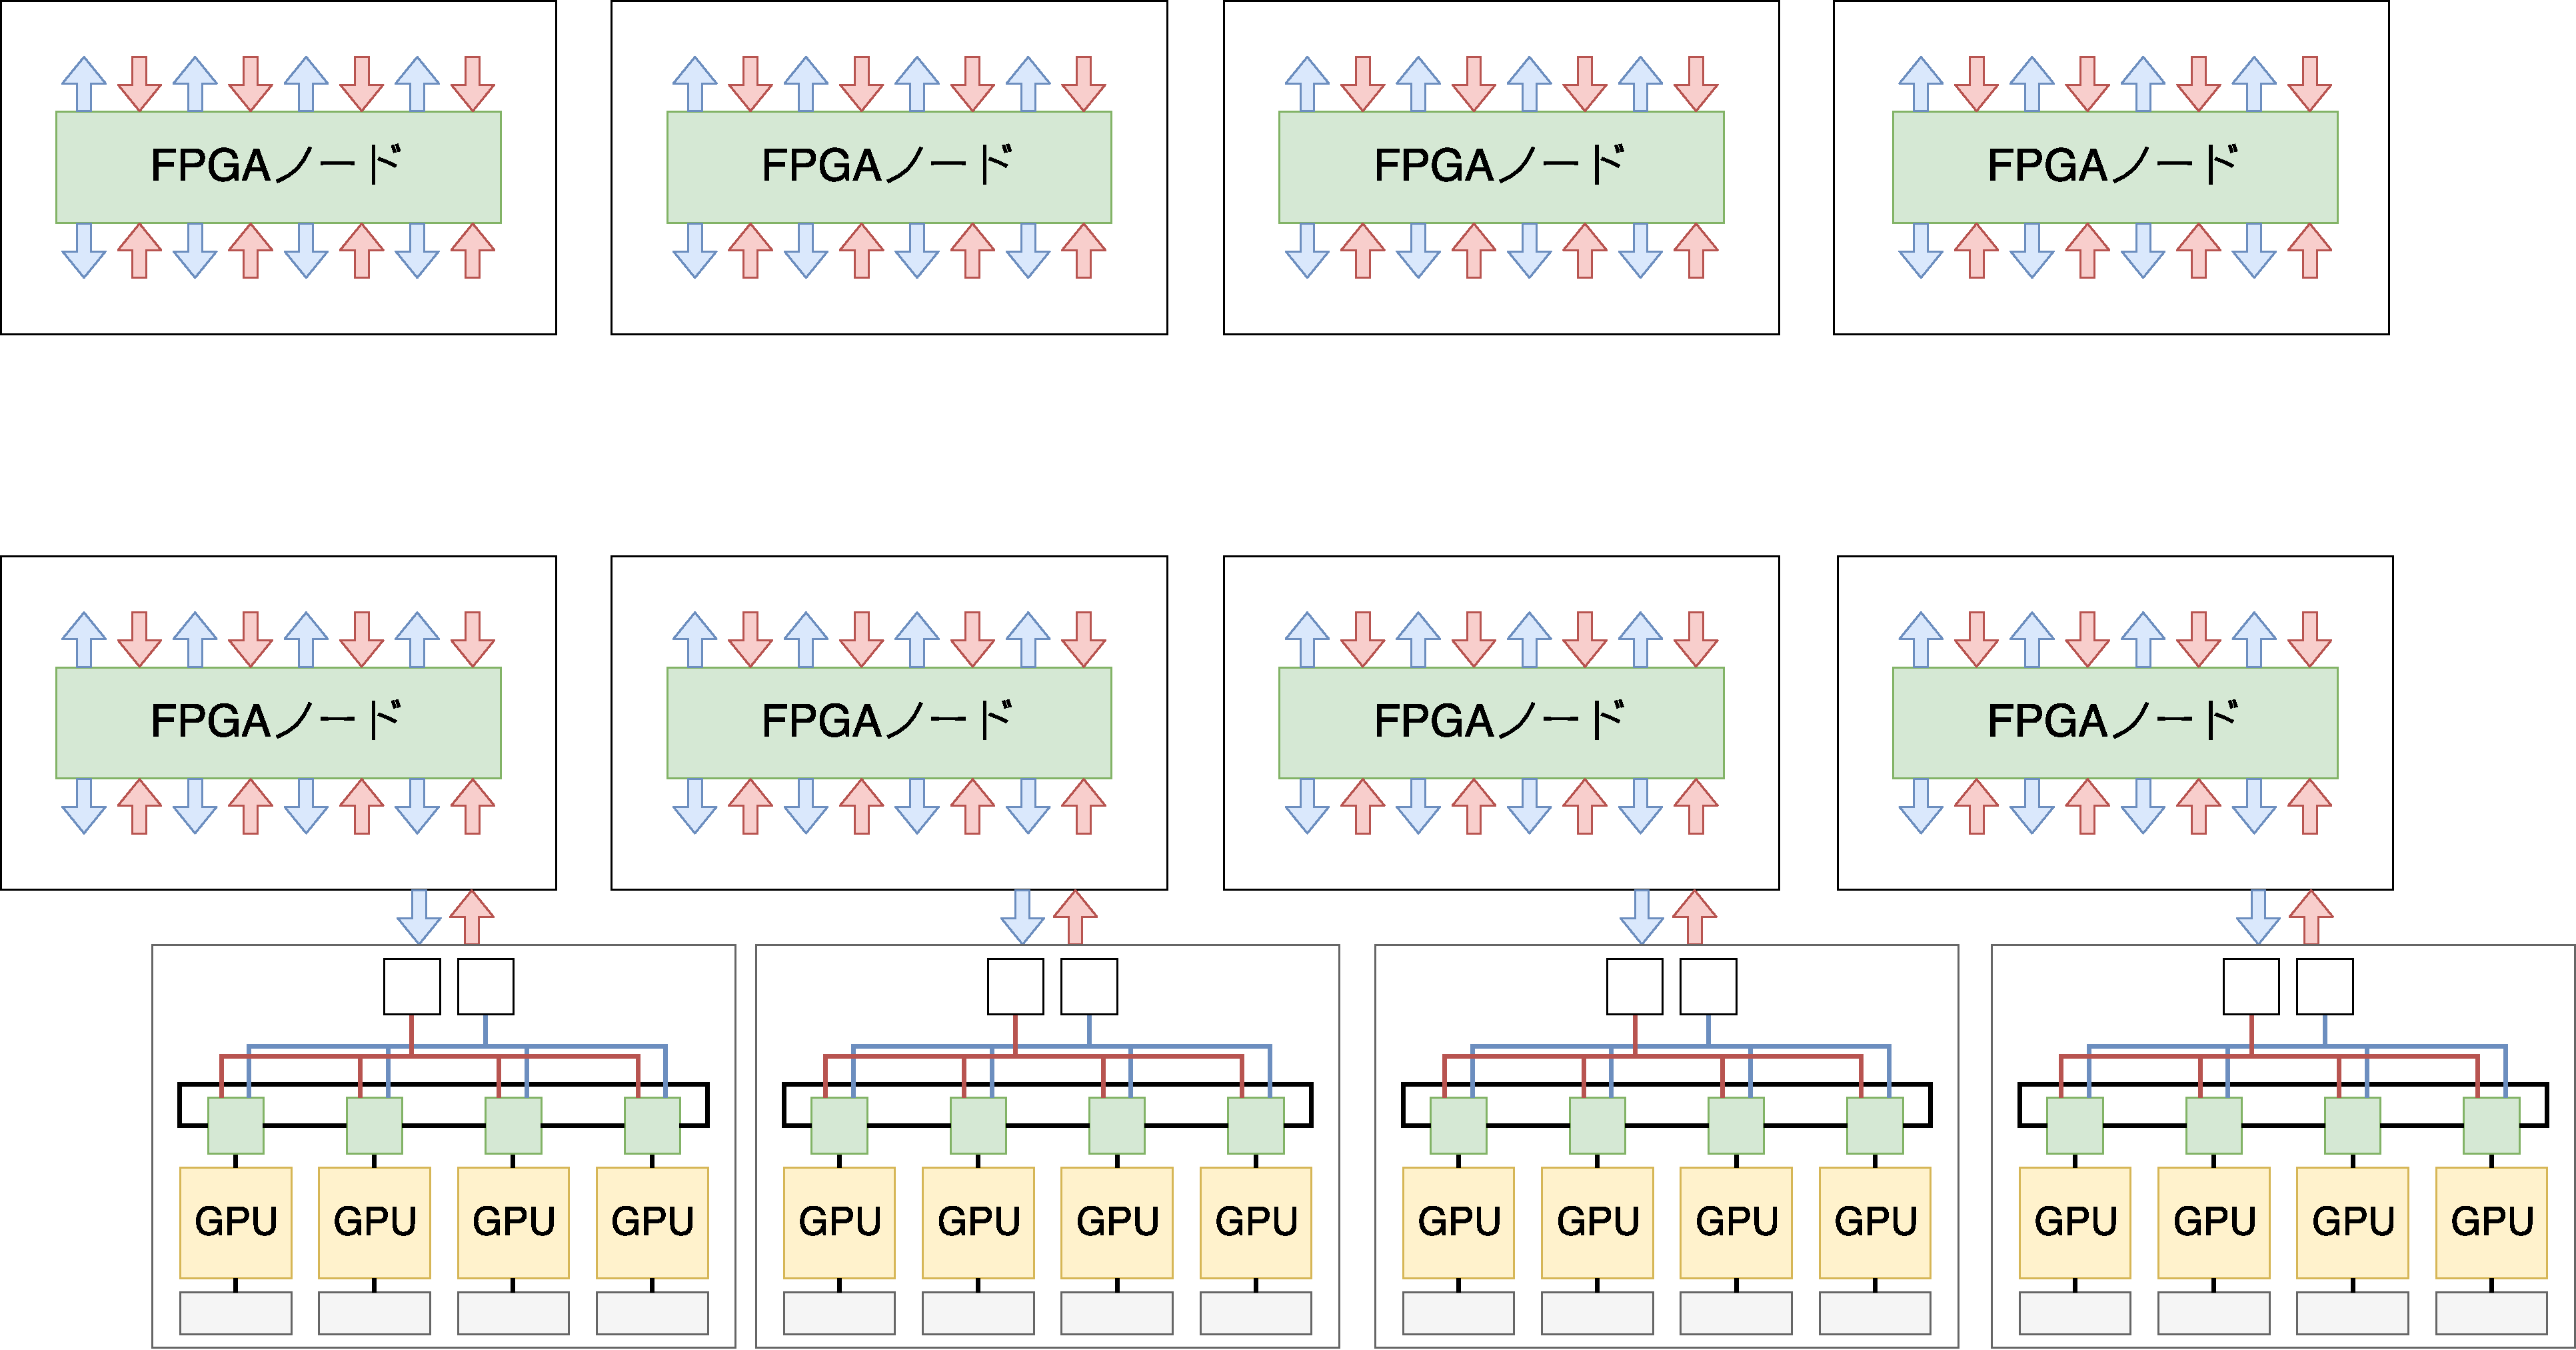
\includegraphics[width=15cm]{./chap3/fig/arch_fic.pdf}
    \caption{FiCのアーキテクチャ}
    \label{fig:arch_fic}
  \end{figure}
  
  FPGAはシステムにおいて高機能スイッチノードとしての役割が期待され,
  他のFPGAやGPU,メモリノードと接続されることでGPU間の高速通信を実現するとともに
  FPGAにプログラムされたデータ処理機構などを組み込むことでホストプロセッサの介在を不要とする.
  メモリノードはFPGAノードに接続されることで,個々のGPUに大容量DRAMをもたせる必要がなくなり,GPUデバイスへのメモリコピーを
  なくすことができ,メモリの利用効率を向上させることができる.
  
  \section{FiC-SWの概要}
  \label{sec:about_ficsw}
  FiCにおいて高機能スイッチとなるFPGAボードはFiCSWと名付けられ,その試作ボードは図\ref{fig:ficsw}である.
  
  \begin{figure}[h]
    \centering
    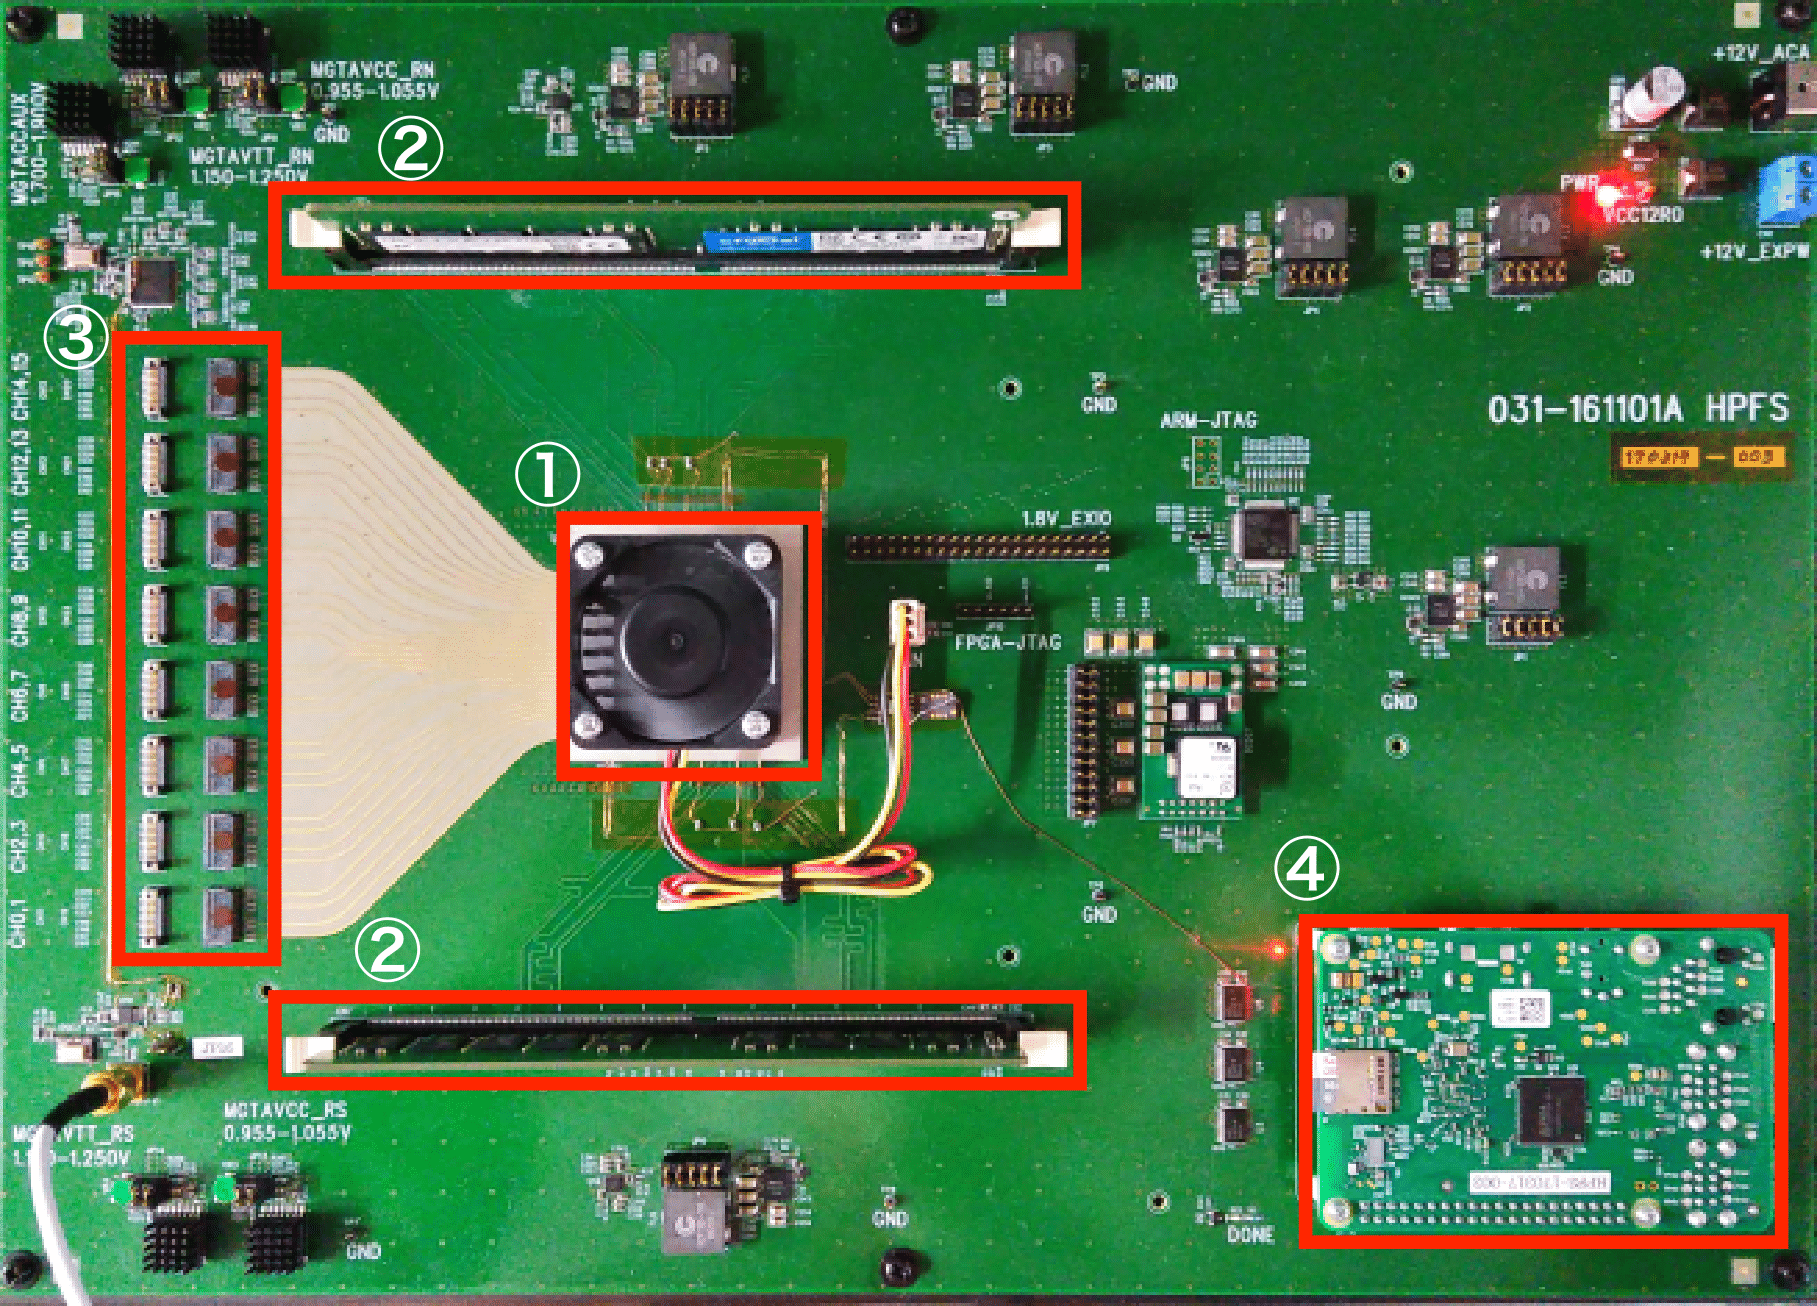
\includegraphics[width=12cm]{./chap3/fig/ficsw.png}
    \caption{FiC-SWの試作ボード}
    \label{fig:ficsw}
  \end{figure}
  
  図\ref{fig:ficsw}中に赤枠で囲まれた4つの要素で構成されている.
  図の注釈の順に
  \begin{enumerate}
    \item Xilinx社製のUltraScale XCKU095-FFVB2104
    \item 高速シリアルリンク8チャネル,32リンク
    \item 16GBのDRAM2バンク
    \item Raspberry Pie3
  \end{enumerate}
  を搭載している.Raspberry Pie3を用いることで,FPGAを遠隔操作して動的に再構成することができる.
  
  \section{FiC-SWでの通信様式}
  \label{sec:ficsw_communication}
  FiCでは将来的に広帯域光通信技術をシステムの相互接続ネットワークに用いることが想定されている.
  光信号のままスイッチすることで数十Tbpsの性能をもつインターコネクトをコストを抑えながらクラウド内で利用する
  ことができる.
  光信号はサーキットスイッチを用いることが現実的である.
  今回のボードは従来の電気信号による通信を行うが来たる光通信の将来を想定して,サーキットスイッチによるネットワークを構成する.
  サーキット数を増やすために時分割多重(TDM: Time Division Mutipling)による通信様式をとる.
  
  図\ref{fig:arch-sw}は4リンクからなるシリアル入力から同じく4リンクからなるシリアル出力へのスイッチの模式図である.
  各リンクが4スロットを有していると仮定している.図中に示される入力スロットと出力スロットの接続が回線を確立する.
  図の破線矢印で示されるように1スロットから複数スロットへの出力を設定することも可能なので,
  容易にブロードキャストを行える.
  各スロットはTDMにより順にデータが入ってくる.
  
   \begin{figure}[h]
     \centering
     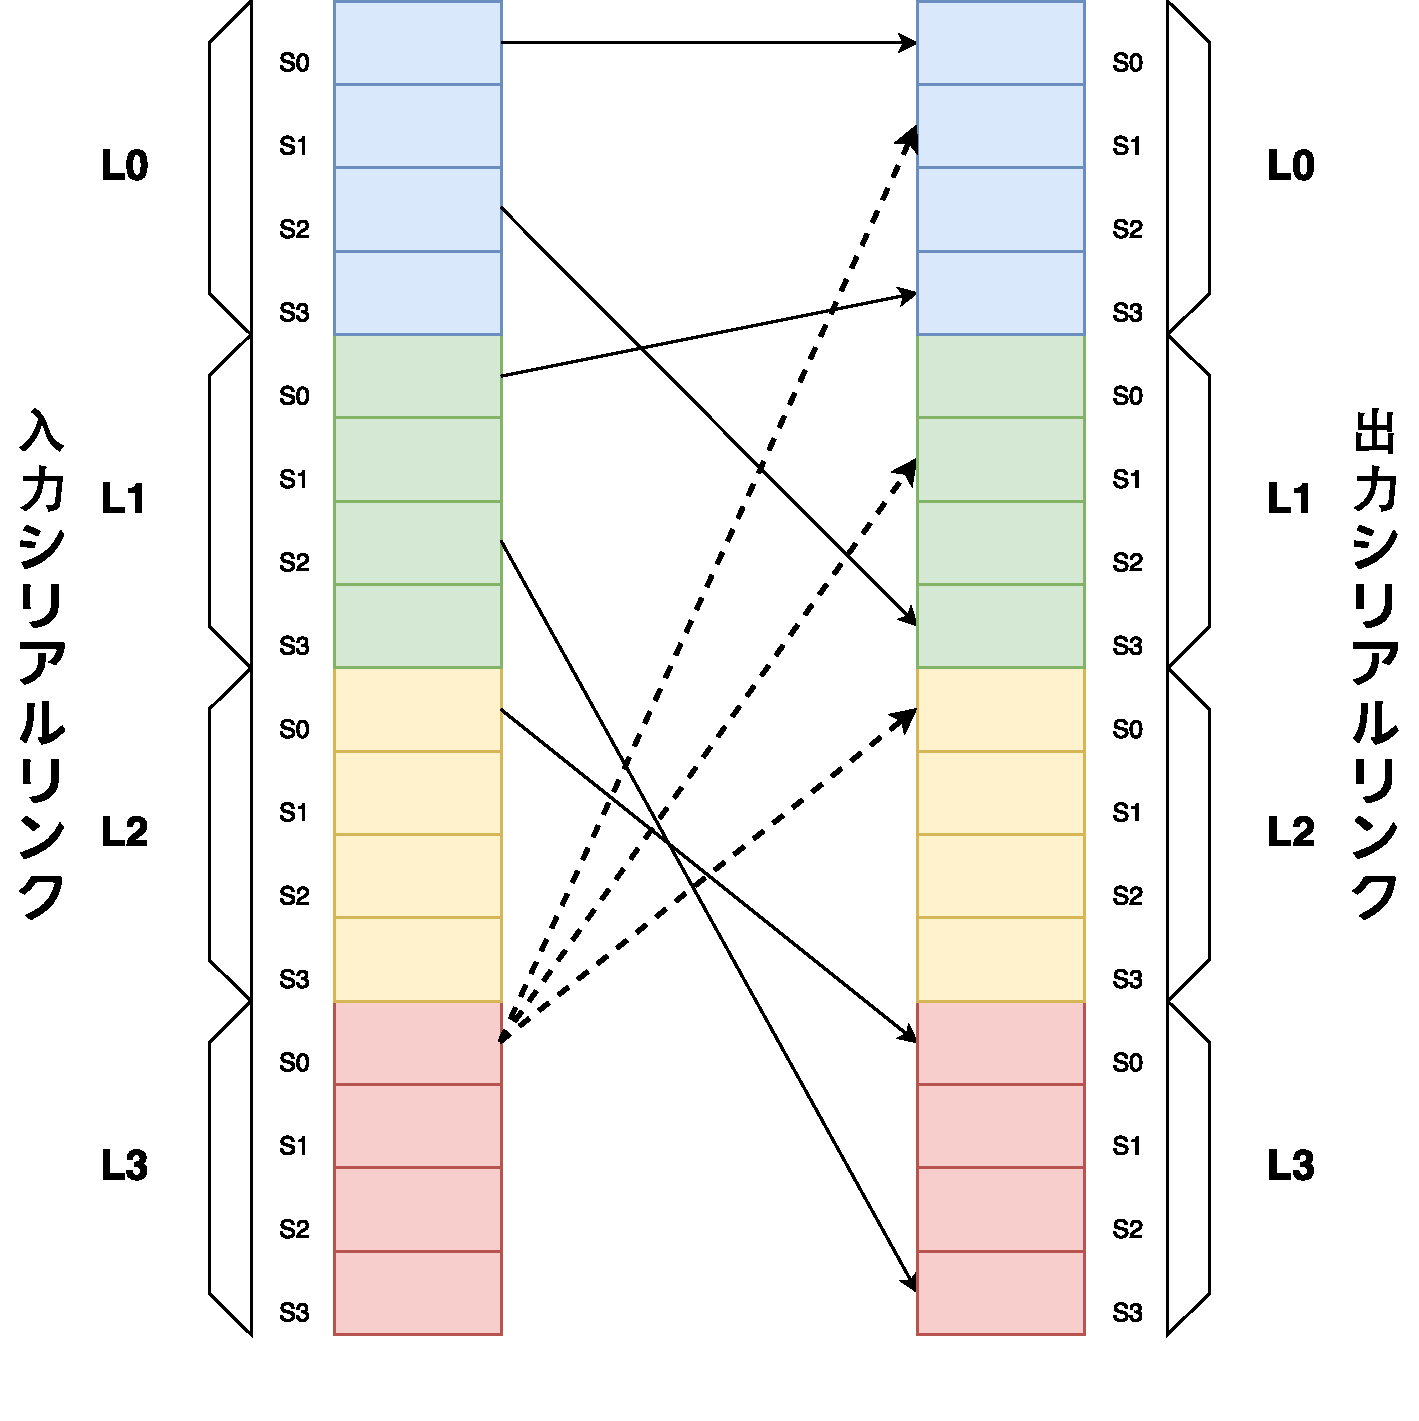
\includegraphics[width=12cm]{./chap3/fig/arch_sw.pdf}
     \caption{FiCのアーキテクチャ}
     \label{fig:arch-sw}
   \end{figure}
}
